Im Folgenden sind die während des Versuchs aufgenommenen Messwerte und die aus diesen 
berechneten Größen tabellarisch dargestellt. An entsprechender Stelle sind Erklärungen
zu den zu den Werten und Rechnungen gegeben.\\

\subsection{Bestimmung der Verdampfungswärme\\ bei Drücken unter einem bar}
	In \autoref{tab:DataI} sind die, für diese Auswertung verwendeten, Messwerte für Temperatur und 
	Druck dieses Teilversuches zu finden. Dabei sind die angegebenen Messunsicherheiten der Temperaturen
	durch die Einteilung Skala des Thermometers und die Unsicherheiten der Drücke durch die Anzeigegenauigkeit 
	des verwendeten Barometers bestimmt. Letztere änderte sich im Verlauf des Versuchs, beziehungsweise
	musste im Verlauf des Versuchs angepasste werden, da sich die Fluktuation der auf dem Barometer angezeigten
	Messwerte vergrößerte.  
	
		\begin{table}[!h]
			\centering
			\begin{tabular}{|c|c||c|c|}
				\hline
				    Temperatur      &       Druck       &      Temperatur      &       Druck       \\
				$T\,[\si{\kelvin}]$ & $p\,[\si{mbar}] $ & $ T\,[\si{\kelvin}]$ & $ p\,[\si{mbar}]$ \\ \hline\hline
				   \num{333(1)}     &   \num{244(1)}    &     \num{353(1)}     &   \num{467(1)}    \\
				   \num{335(1)}     &   \num{260(1)}    &     \num{355(1)}     &   \num{506(10)}   \\
				   \num{337(1)}     &   \num{275(1)}    &     \num{357(1)}     &   \num{553(10)}   \\
				   \num{339(1)}     &   \num{291(1)}    &     \num{359(1)}     &   \num{591(10)}   \\
				   \num{341(1)}     &   \num{310(1)}    &     \num{361(1)}     &   \num{643(10)}   \\
				   \num{343(1)}     &   \num{332(1)}    &     \num{363(1)}     &   \num{694(10)}   \\
				   \num{345(1)}     &   \num{349(1)}    &     \num{365(1)}     &   \num{747(10)}   \\
				   \num{347(1)}     &   \num{374(1)}    &     \num{367(1)}     &   \num{796(10)}   \\
				   \num{349(1)}     &   \num{400(1)}    &     \num{368(1)}     &   \num{821(10)}   \\
				   \num{351(1)}     &   \num{429(1)}    &     \num{369(1)}     &   \num{851(10)}   \\ \hline
			\end{tabular}
			\caption{Werte der Messung bei $p < \SI{1}{bar}$ \label{tab:DataI}}
		\end{table}
	
	Diese Messwerte sind zusammen mit einer Regressionskurve der Form \eqref{eq:pT_exp} in \autoref{fig:pT1}
	aufgetragen, die wegen der halblogarithmischen Skalierung und der Definition $x := \tfrac{1}{T}$ eine Gerade 
	der Form \eqref{eq:pT_ln} darstellt.

	\begin{figure}[!h]
		\centering
		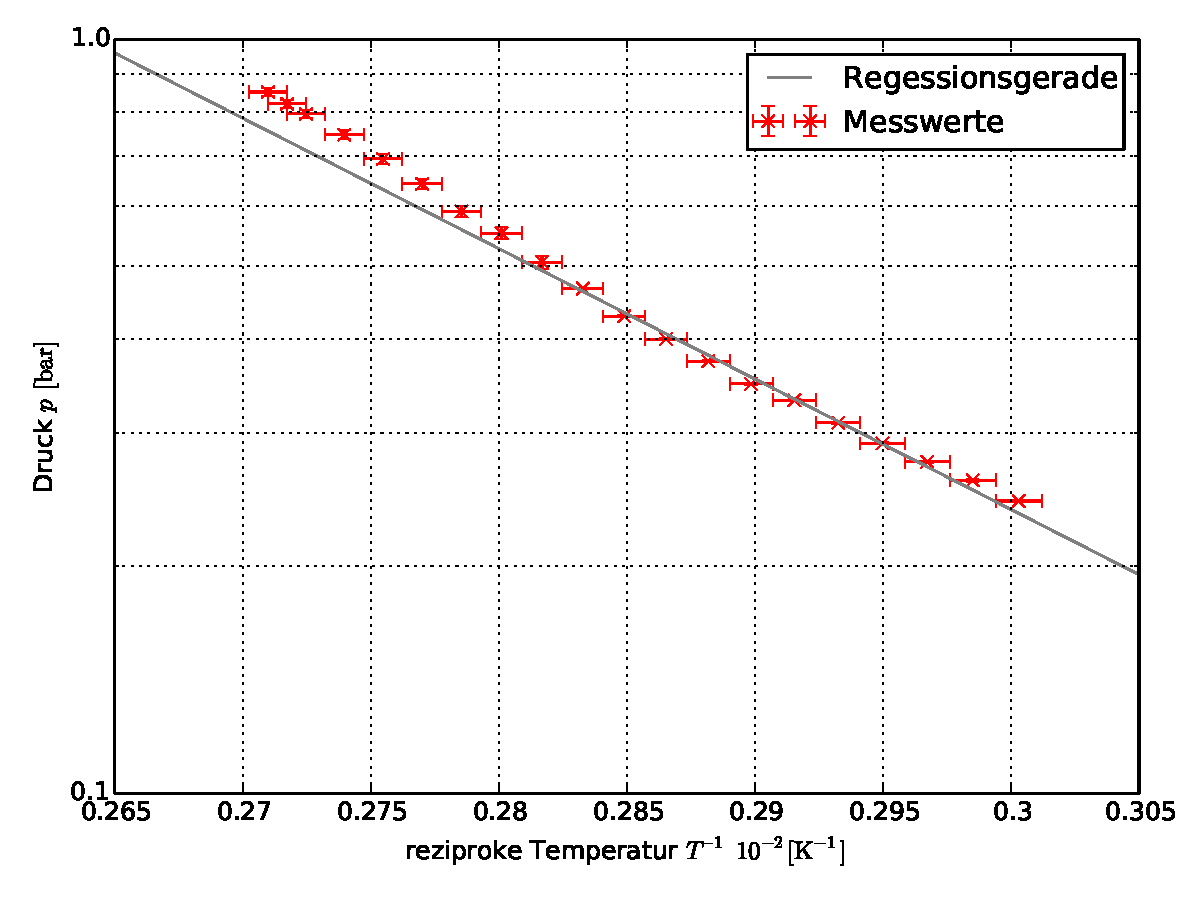
\includegraphics[scale=0.75]{Grafiken/Messreihe_1.pdf}
		\caption{Halblogarithmische Darstellung der Messwerte mit Regressionsfunktion}
		\label{fig:pT1}
	\end{figure}   
	
	Die mit Hilfe der Python Bibliothek \emph{SciPy} \cite{SciPy} bestimmten Parameter dieser der Regerssionsfunktion $f(x) = A + Bx$ sind:
	\begin{subequations}
		\begin{empheq}{align}
			\label{eq:A}
			A &= \SI{11(9)}{\bar}\\
			\label{eq:B}
			B &= \SI{-0.040(1)}{\bar\kelvin}
		\end{empheq}
	\end{subequations} 
	
	 Mit $B = - \tfrac{L}{R}$ und der allgemeinen Gaskonstante $R = \SI{8.314}{\joule\per\mol\per\kelvin}$  \cite{SciPy} lässt
	 sich die Verdampfungswärme aus der Steigung \eqref{eq:B} zu
	 
	\begin{empheq}{equation*}
	 		\label{eq:L}
	 		L = \SI{3.31(8)e04}{\joule\per\mole}
	\end{empheq}
	berechnen.
	
	\subsection{Bestimmung der inneren Verdampfungswärme}
	Für die äußere Verdampfungswärme $L_{a}$ erhält man unter Verwendung der allgemeinen
	Gasgleichung \eqref{eq:allgGas} und der Annahme $V_{D} >> V_{F}$ die Näherung
	\begin{empheq}{equation}
	 	\label{eq:L_a}
	 	L_{a} = RT.
	\end{empheq}
	Bei der gegebenen Temperatur $T = \SI{373}{\kelvin}$ ergibt sich damit die notwendige 
	Energie, um das Volumen $V_{F}$ auf $V_{D}$ zu vergrößern zu
	\begin{empheq}{equation*}
		 	L_{a} =  \SI{3101}{\joule\per\mole}\;.
    \end{empheq}  
	Aus der gesamten $L$ und  äußeren Verdampfungswärme $L_{a}$ lässt sich mit \eqref{eq:L_i}
	die innere Verdampfungswärme bestimmen. Durch Skalierung mit der Avogadro-Konstante 
	$N_{A} = \SI{6.022e23}{\per\mole}$ \cite{SciPy} und Umrechnung in $\si{\eV}$\footnote{\si{\eV} = \SI{1.602e-19}{\joule} \cite{SciPy}},
	erhält man die für die Verdampfung eins einzelnen Wassermoleküls benötigte Energie
	\begin{empheq}{equation*}
			 	L_{i} =  \SI{0.331(8)}{\eV}\;.
	\end{empheq} 
	
	
\subsection{Bestimmung der Temperaturabhängigkeit\\ der Verdampfungswärme}